\chapter{Preparation}

\section{Design of an awesome resonator}

\section{Measuring the Resonator Parameters}

\begin{figure}[h]%
\centering
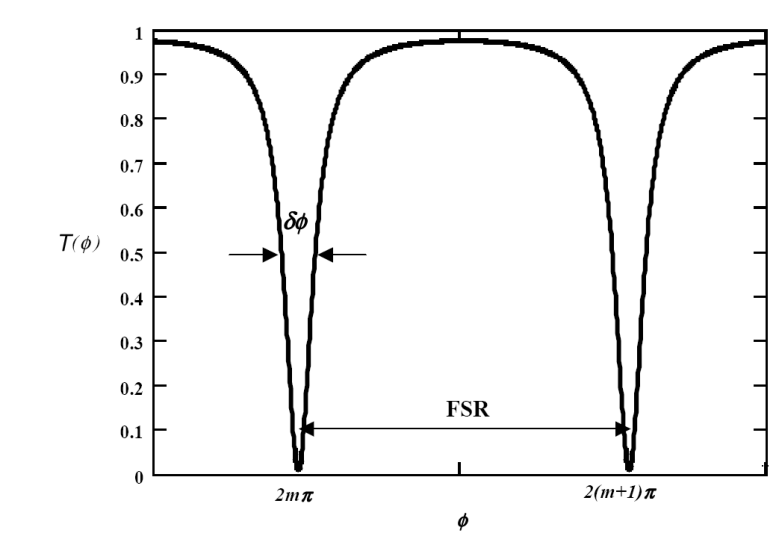
\includegraphics[width=.5\columnwidth]{Grafiken/S21.pdf}%
\caption{Example Transmission Coefficient of a Resonator}%
\label{fig:S21}%
\end{figure}
\todo{Bild evtl auf f anpassen}

To caracterize a resonator its power transmission in dependency of the frequency can easily be measured. By that measurement, the whidth of the resonance lines at full width half maximum (FWHM) $\delta f$ and the free spectral range $\Delta f$ can determined. (cf. figure \ref{fig:S21}). The quotient $F= \Delta f/\delta f$ is called Finesse. For the case of critical coupling $F$ is given as:
\begin{equation}
 F = \frac{\Delta f}{\delta f} = \frac{\pi\sqrt{1-\kappa}}{\kappa}=\frac{\pi\exp\left(-\alpha/2L\right)}{1-\exp\left(-\alpha/L\right)}
\end{equation}
This can be rearranged to:
\begin{equation}
 \kappa = 0.5 \pm \sqrt{0.25+F^2/\pi^2}
\end{equation}
and
\begin{equation}
\alpha = -\frac{\ln F}{L(\ln F+2\ln\pi)} 
\end{equation}
respectively.

\section{Over-Critical and Under-Critical coupling}